\chapter{Project Details}

This chapter provides an in-depth explanation of the project's components and tools used. The system was developed using Swift, Xcode, and RealityComposer Pro to leverage the capabilities of Apple Vision Pro.

% \section{UI/UX Design}
\section{UI/UX Design}

The application has a streamlined user interface with a single window navigating between different views to ensure an intuitive and user-friendly experience. Below is the flow of UI/UX interactions:

\subsection{Initial Session Start}
The application starts with a view prompting the user to begin an ARKit session. This session initializes plane detection and world tracking. The interface provides visual indicators to guide the user during this setup phase. (Figure \ref{fig:ui_session_start} shows the UI at this stage.)
\begin{figure}[h!]
    \centering
    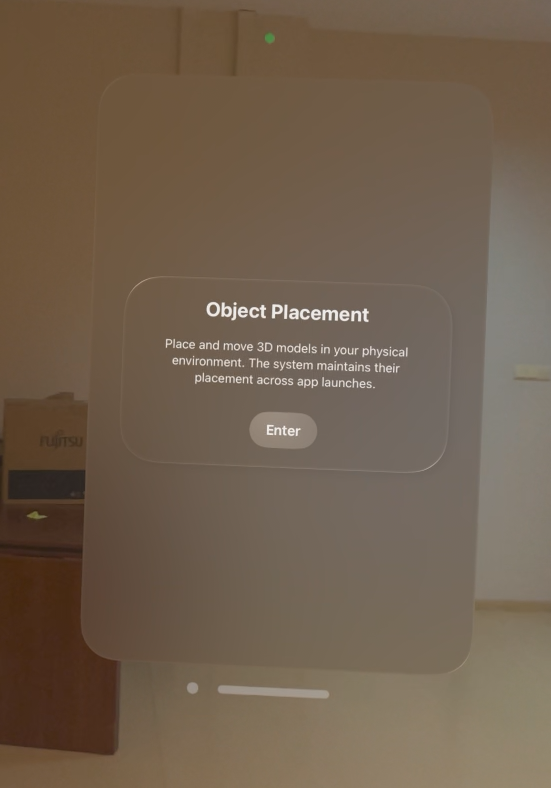
\includegraphics[width=0.4\textwidth]{session_start_ui.png} % Replace with your image file name
    \caption{UI for starting the ARKit session.}
    \label{fig:ui_session_start}
\end{figure}
\subsection{Object Selection Menu}
After initializing the session, the user is directed to an object selection menu. In this view:
\begin{itemize}
    \item The user selects an object from the available options.
    \item When an object is clicked, the \texttt{selectedObject} state is updated.
    \item The selected object is prepared for placement. (Figure \ref{fig:ui_object_selection} shows the object selection menu.)
\end{itemize}
\begin{figure}[h!]
    \centering
    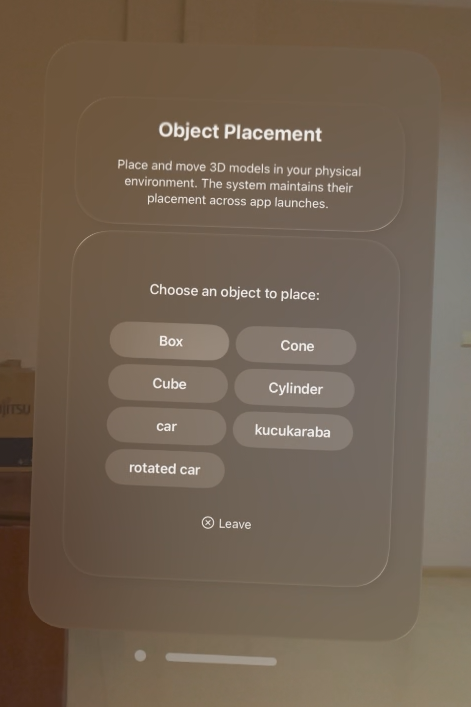
\includegraphics[width=0.4\textwidth]{object_selection_ui.png} % Replace with your image file
    \caption{Object selection menu UI.}
    \label{fig:ui_object_selection}
\end{figure}

\subsection{Initial Object Placement}
During the initial placement of the selected object:
\begin{itemize}
    \item Placement tooltips are displayed to guide the user on positioning the object accurately.
    \item Visual aids ensure the user understands how to interact with the AR environment. (Figure \ref{fig:ui_initial_placement} shows the placement tooltip.)
\end{itemize}
\begin{figure}[h!]
    \centering
    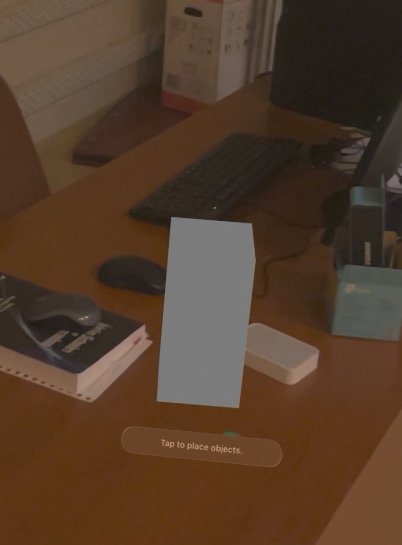
\includegraphics[width=0.4\textwidth]{object_placement_tooltips.png} % Replace with your image file
    \caption{Placement tooltips during initial object placement.}
    \label{fig:ui_initial_placement}
\end{figure}


\subsection{Object Interaction View}
If there is already a placed object, the application navigates directly to the object interaction view. In this view:
\begin{itemize}
    \item The user can perform repositioning, inspection, or removal of the placed object. The interface displays three buttons for these actions, as shown in Figure \ref{fig:ui_three_buttons}.
    \begin{figure}[h!]
        \centering
        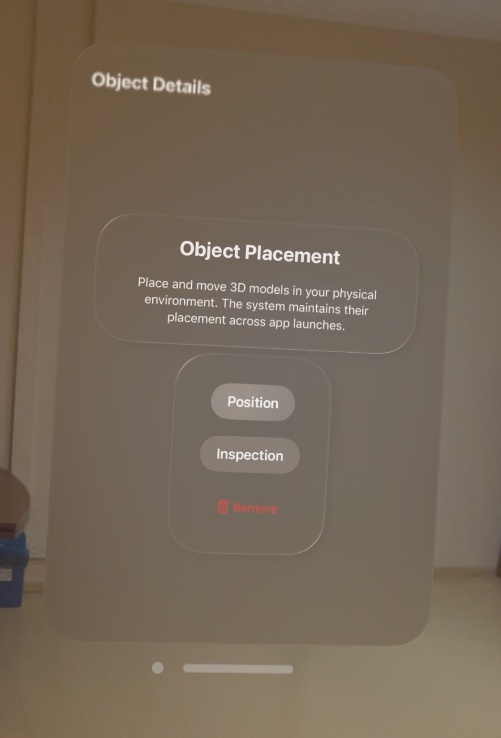
\includegraphics[width=0.39\textwidth]{three_buttons_ui.png} % Replace with the actual file name
        \caption{UI showing the three buttons for repositioning, inspection, and removal.}
        \label{fig:ui_three_buttons}
    \end{figure}
    \clearpage
    \item Three buttons allow the user to activate these actions:
    \begin{itemize}
        \item \textbf{Repositioning:} Includes rotation, left/right movement, and forward/backward movement. The user can use pinch and drag gestures (thumb and index finger) to perform the action. Only one action can be performed at a time. (Figure \ref{fig:ui_repositioning} shows the repositioning process.)
        \begin{figure}[h!]
            \centering
            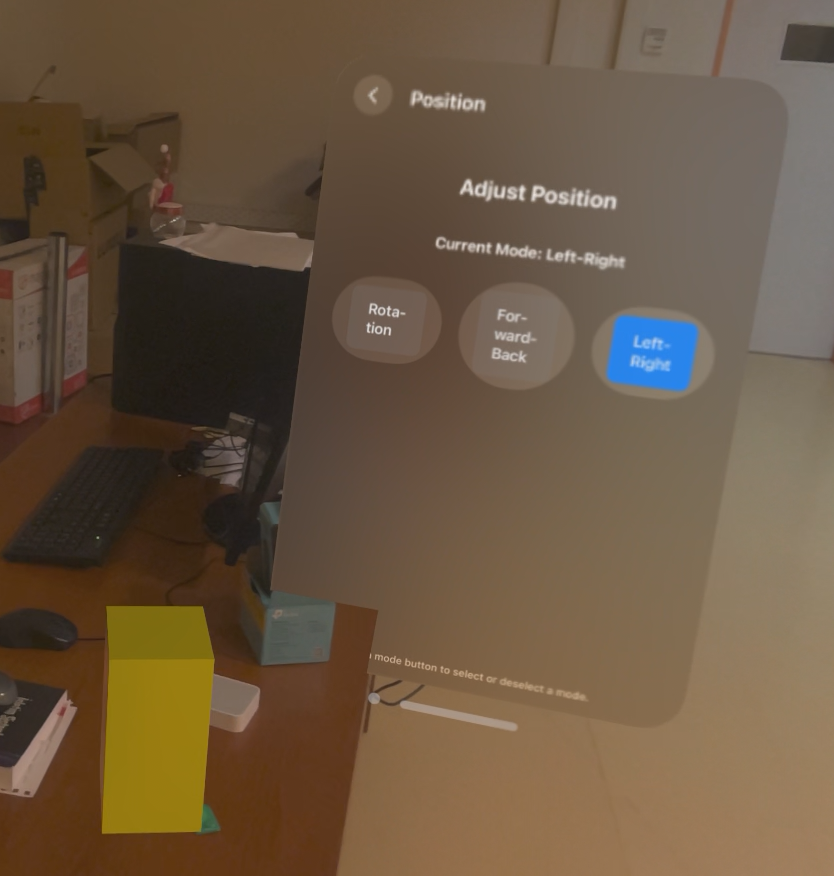
\includegraphics[width=0.6\textwidth]{repositioning_ui.png} % Replace with the actual file name
            \caption{Repositioning the object using pinch and drag gestures.}
            \label{fig:ui_repositioning}
        \end{figure}
        \item \textbf{Inspection:} Inspection points are UI buttons attached to the placed object. These points activate only in the inspection view. In addition, the inspection view includes a \textbf{Generate Report} button, allowing the user to extract detailed quality analysis reports based on the performed inspections. (Figure \ref{fig:ui_inspection_view} shows the inspection view.)
        \clearpage
        \begin{figure}[h!]
            \centering
            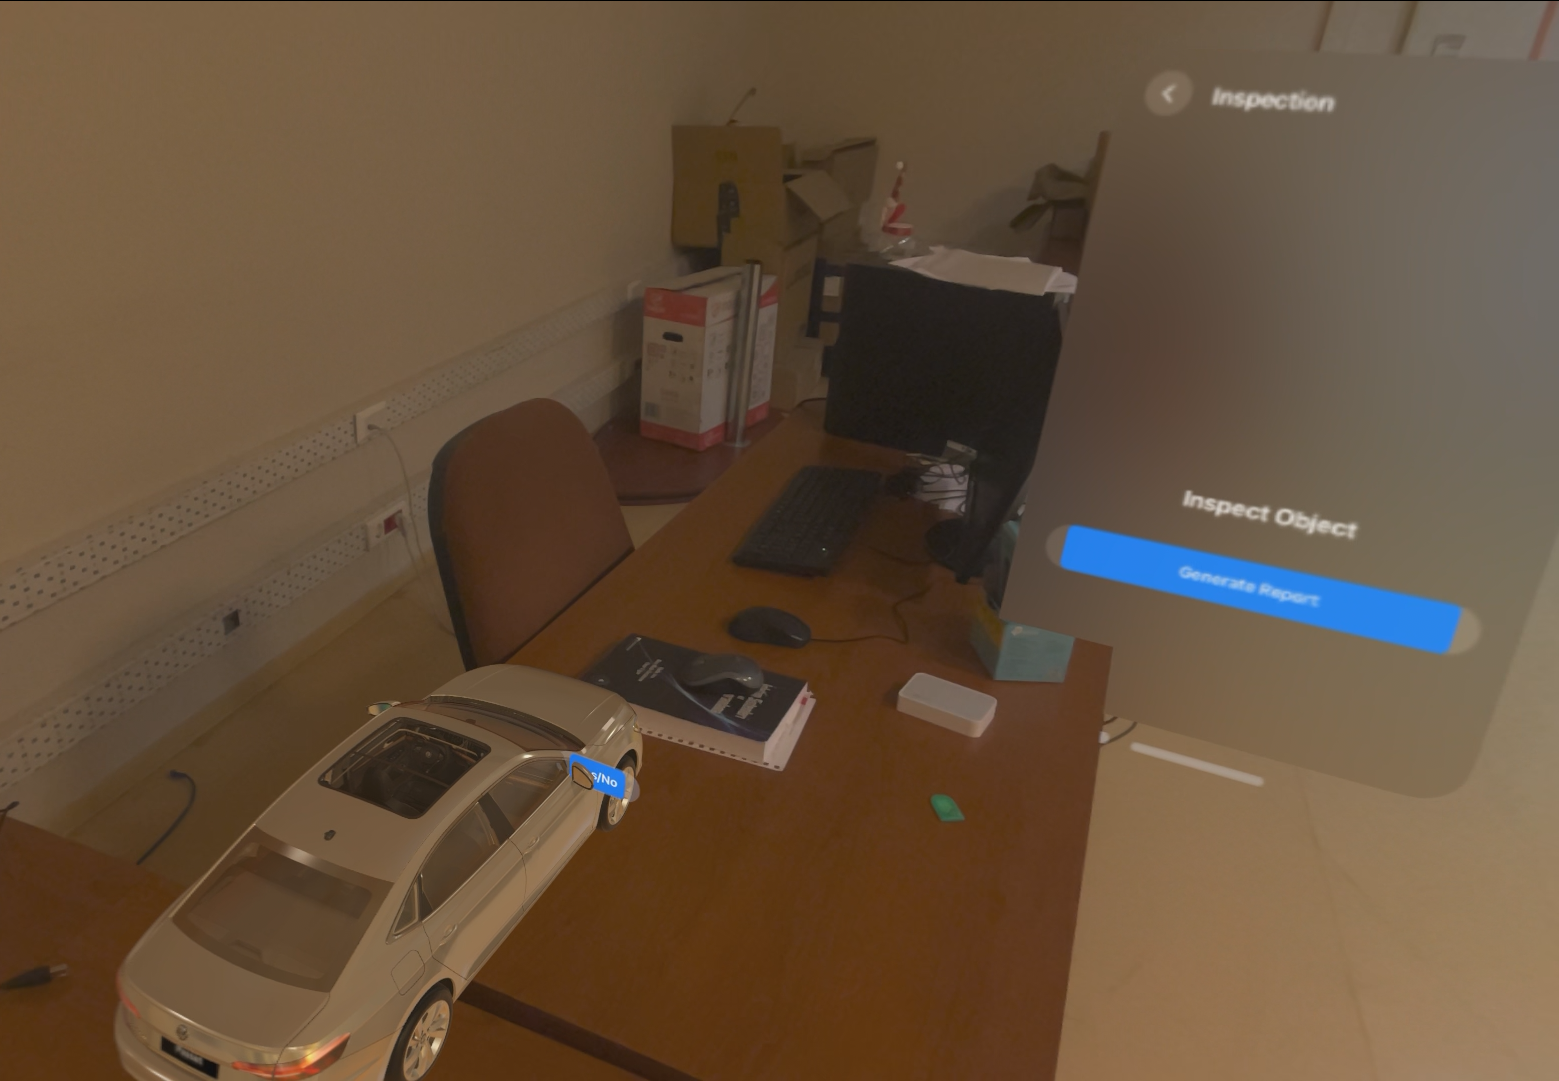
\includegraphics[width=0.8\textwidth]{inspection_view_ui.png} % Replace with the actual file name
            \caption{Inspection view showing active inspection points.}
            \label{fig:ui_inspection_view}
        \end{figure}
        \item \textbf{Removal:} To remove the placed object, the user presses the remove button. A confirmation popup appears to ensure the action is intentional. (Figure \ref{fig:ui_remove_popup} shows the removal confirmation popup.)
        \begin{figure}[h!]
            \centering
            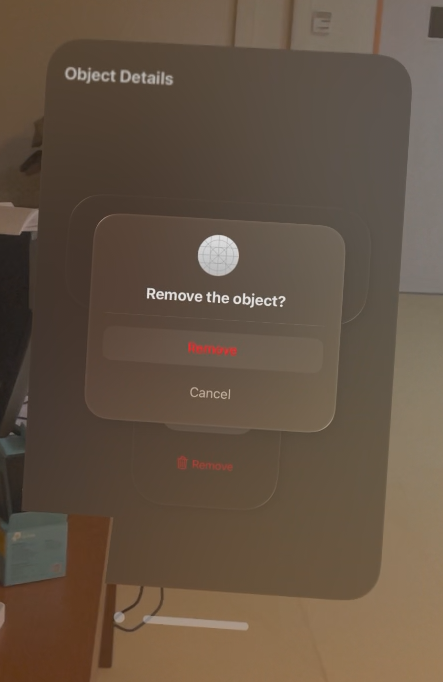
\includegraphics[width=0.4\textwidth]{remove_popup_ui.png} % Replace with the actual file name
            \caption{Confirmation popup for removing the placed object.}
            \label{fig:ui_remove_popup}
        \end{figure}
    \end{itemize}
\end{itemize}

\subsection{Inspection Detail View}
When an inspection point is clicked, the application navigates to the inspection detail view:
\begin{itemize}
    \item A question specific to the inspection point is displayed, which can be one of the following:
    \begin{itemize}
        \item Yes/No question.
        \item Count input.
        \item Description input.
    \end{itemize}
    \item The user provides the required input or feedback. (Figure \ref{fig:ui_inspection_detail} shows the inspection detail view.)
\end{itemize}

\begin{figure}[h!]
    \centering
    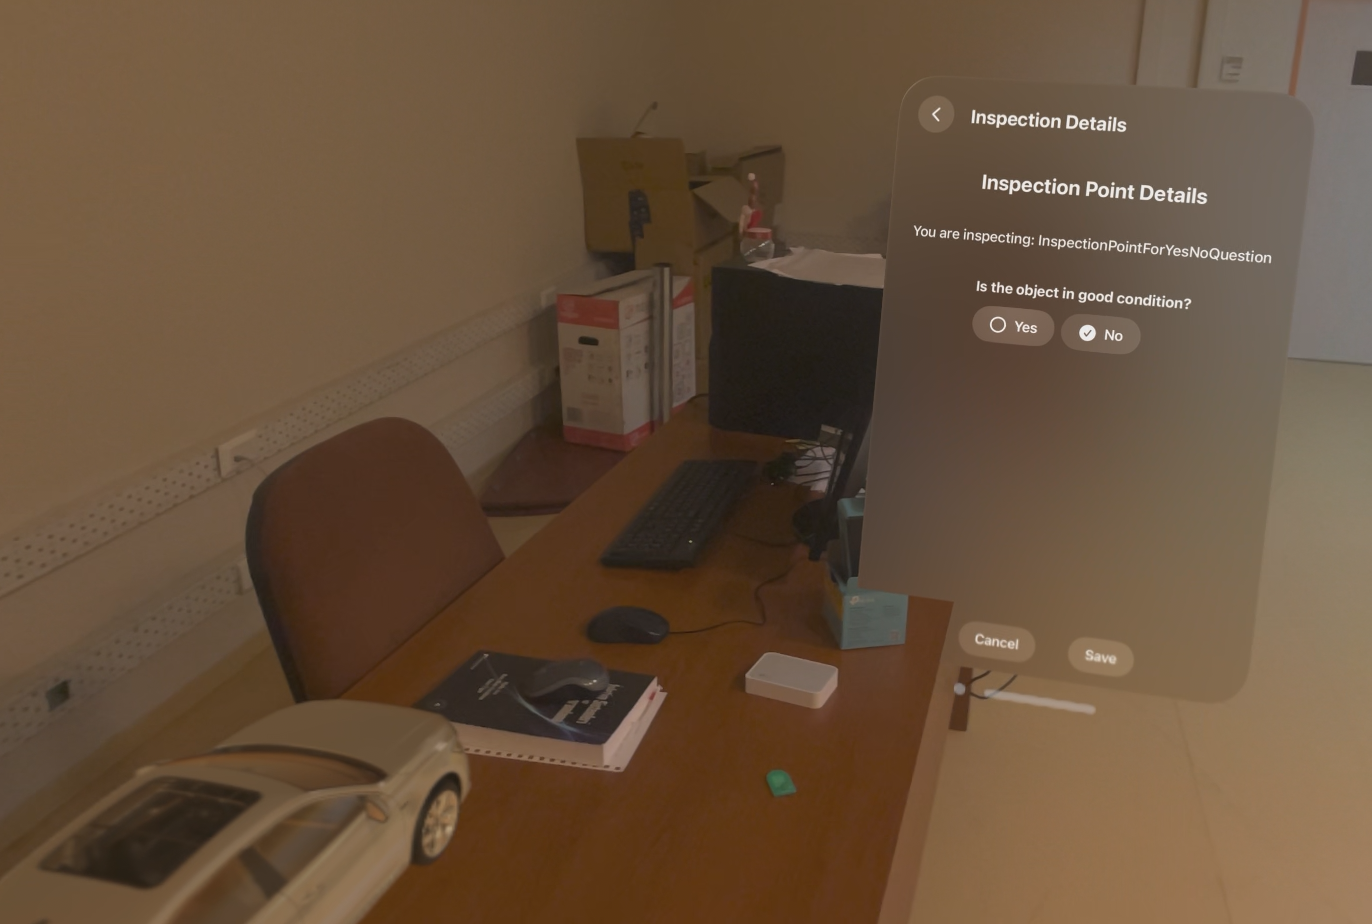
\includegraphics[width=0.8\textwidth]{inspection_detail_ui.png} % Replace with your actual file name
    \caption{Inspection detail view showing specific question types and input fields.}
    \label{fig:ui_inspection_detail}
\end{figure}


\section{Model Alignment and Placement}

The system leverages ARKit’s capabilities for world tracking and plane detection to enable accurate model alignment and placement. Horizontal planes are specifically chosen to detect ground planes, ensuring precise object placement in the AR environment.

The 3D models used in the application are in the USDZ format, which is optimized for AR experiences on Apple devices.
\subsection{Initial Placement}
During initial placement, the user is provided with a preview of the selected object. The preview is displayed as a greyed-out version of the object accompanied by a placement tooltip to guide the user in positioning it accurately. This feature allows the user to visually align the object with the detected ground plane before finalizing its placement, as shown in Figure \ref{fig:ui_initial_placement}.

To ensure that objects fit appropriately within the environment, size adjustments are made to the USDZ 3D models using SceneKit. 
\subsection{Replacement}
If the user needs to reposition an already placed object, they can do so in the position mode of the application. In this mode:
\begin{itemize}
    \item The user can perform object rotation, as well as left/right and forward/backward movements.
    \item These adjustments are enabled only when the position mode is activated in the position view.
    \item Pinch and drag gestures (thumb and index finger) are used to perform these actions, as shown in \ref{fig:ui_repositioning}.
\end{itemize}

By combining ARKit’s robust plane detection with intuitive interaction methods, the system ensures precise and user-friendly model alignment and placement.


% Explanation about inspection will go here.
\section{Inspection}

All inspection operations, including exporting reports, providing input to inspection points, or viewing inspection points, occur exclusively within the \textbf{Inspection View}. If the application is not in the \textbf{Inspection View}, all inspection points are removed from the interface. When the user navigates back to the \textbf{Inspection View}, the inspection points are dynamically regenerated. (as shown in Figure \ref{fig:ui_inspection_view})

To prevent user confusion or potential issues (e.g., uncertainty about whether data is saved), all inspection points are also removed when the application navigates to the \textbf{Inspection Detail View}. This design decision ensures reliability and eliminates bugs arising from unclear save states or interactions. (as Shown in Figure \ref{fig:ui_inspection_detail})

\subsection{Inspection Points}
For each inspection point on the placed model, a UI button is displayed (as shown in Figure \ref{fig:ui_inspection_view}). These buttons are dynamically positioned based on the specific locations of the inspection points on the model. When the user clicks an inspection point button, the application navigates to the \textbf{Inspection Detail View}, where the selected inspection point can be reviewed and updated.

\subsection{Inspection Detail View}
In the \textbf{Inspection Detail View}, users can perform inspections on the selected point. The system supports three types of inspections:
\begin{itemize}
    \item \textbf{Yes/No:} A binary choice indicating whether the inspection criteria have been met, as Shown in Figure \ref{fig:ui_inspection_detail}.
    \item \textbf{Count:} Allows the user to input the quantity of specific elements related to the inspection point.
    \item \textbf{Description:} Provides a text field for the user to enter detailed notes or comments about the inspection point.
\end{itemize}

\subsection{Exporting Reports}
The \textbf{Inspection View} includes a \textbf{Generate Report} button, enabling users to export a report of all completed inspections.

By limiting inspection operations to the \textbf{Inspection View} and \textbf{Inspection Detail View}, the system ensures a consistent and reliable user experience while minimizing potential errors or confusion.


% Explanation about generating reports will go here.
\section{Report Generation}

The report generation functionality in this system is powered by the third-party C library \textbf{libxlsxwriter}, which facilitates the creation of Excel files. This feature enables users to export inspection reports, which are saved directly to the Apple Vision Pro's local directory for easy access.

\subsection{Implementation Overview}
Each report file is named dynamically based on the object being inspected and a unique identifier to avoid conflicts.

\subsection{Report Content}
The generated report contains the following key information:
\begin{itemize}
    \item \textbf{Object Details:} The name, width, height, and depth of the inspected object are recorded in the report.
    \item \textbf{Inspection Points:} Each inspection point associated with the object is detailed in the report. For every inspection point, the following attributes are included:
    \begin{itemize}
        \item \textbf{Name:} The identifier of the inspection point.
        \item \textbf{Depending on The Type of Inspection:}
        \begin{itemize}
            \item \textbf{Count:} The quantity associated with the inspection point, if applicable.
            \item \textbf{Description:} Detailed notes or observations provided by the user.
            \item \textbf{Is Correct:} A binary value (Yes/No) indicating whether the inspection point meets the desired criteria.
        \end{itemize}
    \end{itemize}
\end{itemize}

An example of the generated Excel report is shown in Figure \ref{fig:example_excel}.
\begin{figure}[h!]
    \centering
    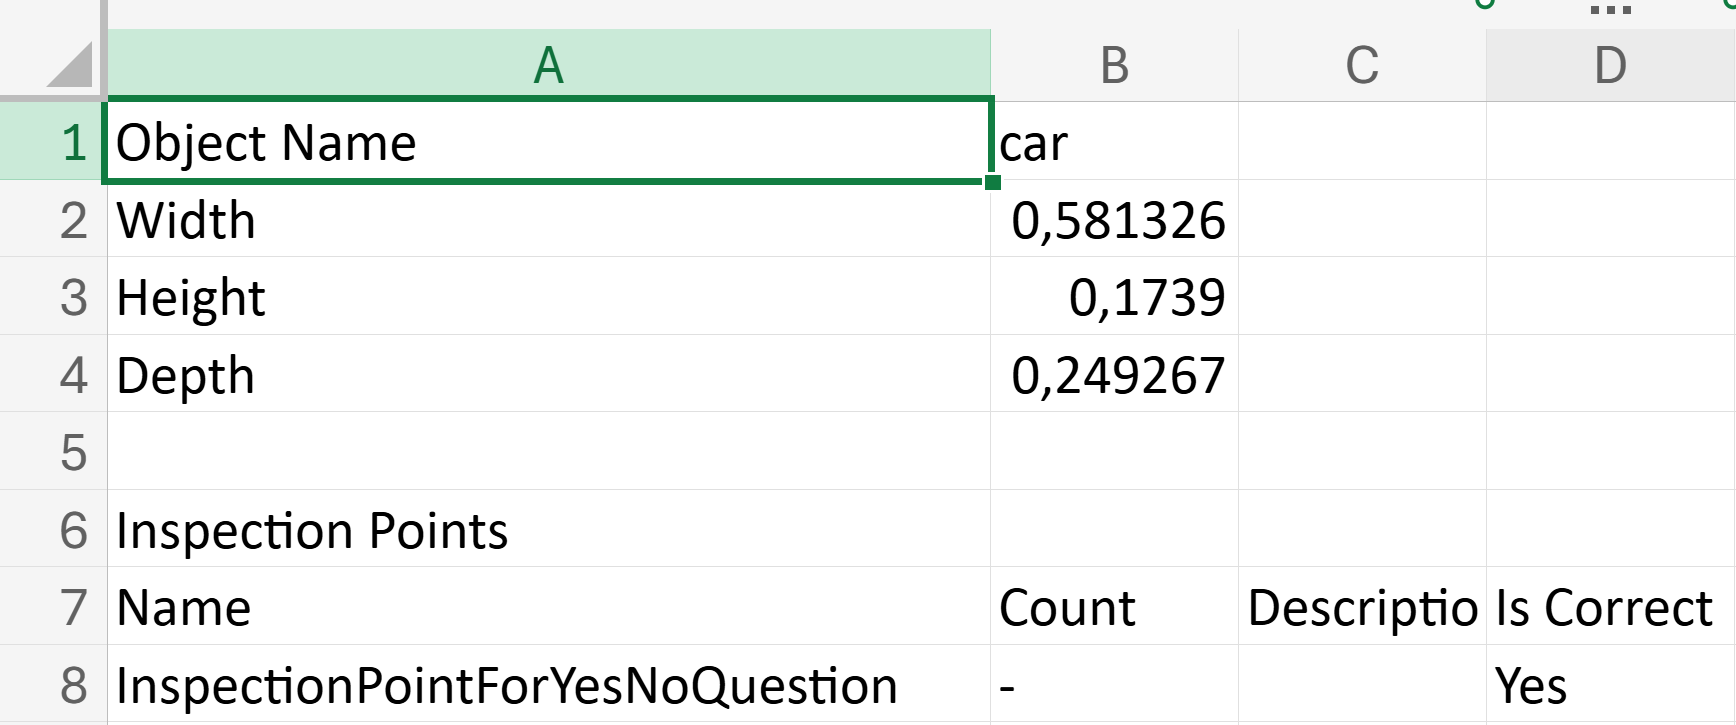
\includegraphics[width=0.8\textwidth]{example_excel.png} % Replace with your actual file name
    \caption{Example Excel report generated by the application.}
    \label{fig:example_excel}
\end{figure}

\subsection{Integration with Apple Vision Pro}
The reports are stored locally on the Apple Vision Pro device, allowing users to access them conveniently through the file system. This integration ensures compatibility with the Vision Pro environment and leverages the device's capabilities for efficient data handling.

By using \textbf{libxlsxwriter}, the system provides a robust and efficient way to generate and manage detailed Excel reports, enhancing the overall functionality and usability of the quality control application.



\section{Use Case Diagram}
The use case diagram below illustrates the interaction between the user and the primary functionalities of the system.

\begin{center}
    \begin{tikzpicture}[node distance=3cm]

        % Actor
        \node (user) [actor] {User};

        % Use cases
        \node (start) [usecase, below of=user, xshift=-6cm] {Start ARKit Session};
        \node (select) [usecase, below of=user, xshift=-2cm] {Select Object};
        \node (place) [usecase, below of=user, xshift=2cm] {Place Object};
        \node (reposition) [usecase, below of=user, xshift=6cm] {Reposition Object};
        \node (inspect) [usecase, below of=user, yshift=-6cm] {Inspect Object};
        \node (provide) [usecase, below of=inspect, xshift=-4cm] {Provide Inspection Input};
        \node (report) [usecase, below of=inspect, xshift=4cm] {Generate Report};

        % Connections between actor and use cases
        \draw [->] (user) -- (start);
        \draw [->] (user) -- (select);
        \draw [->] (user) -- (place);
        \draw [->] (user) -- (reposition);
        \draw [->] (user) -- (inspect);

        % Relationships between use cases
        \draw [->] (inspect) -- node[midway, above] {includes} (provide);
        \draw [->] (inspect) -- node[midway, above] {includes} (report);

    \end{tikzpicture}
\end{center}

